
\section{动态规划}
\label{sec:dynamic-programming}

\begin{example}
  从左下角的格子走到右上角的格子,规定每次只能走一格,且只能往右或者往上走,那么总共有多少种走法?
  \begin{center}
    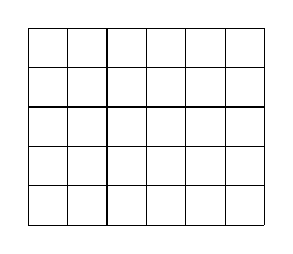
\begin{tikzpicture}[scale=.5]
      \draw(0,0)grid(6,5);
    \end{tikzpicture}
  \end{center}
\end{example}
\begin{proof}[提示]
  显然到达最左边一行与最下面一行的格子都只能有一种走法,可以先填入。
  \begin{center}
    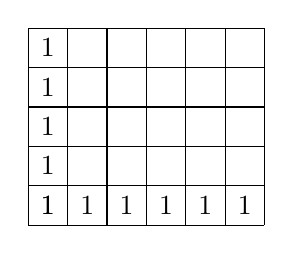
\begin{tikzpicture}[scale=.5]
      \begin{scope}
        \draw(0,0)grid(6,5);
        \foreach \x in{0,1,2,3,4,5}{%
          \node at (\x + .5, .5) {1};
        }
        \foreach \x in{0,1,2,3,4}{%
          \node at (.5, \x + .5) {1};
        }
      \end{scope}
    \end{tikzpicture}
  \end{center}

  考虑其递推关系。容易知道到达一个格子,如果只能用一步的话,那有两种方法,即从其左边的格子到达,或从其下边的格子到达。
  \begin{center}
    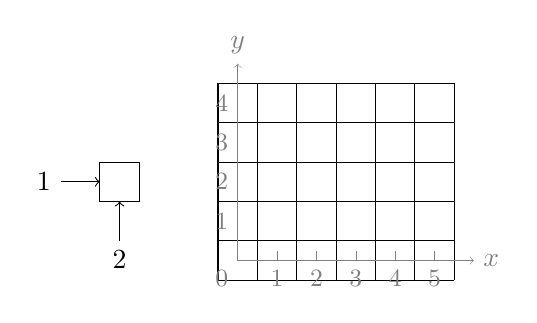
\begin{tikzpicture}[scale=.5]
      \begin{scope}[shift={(0,2)}]
        \draw(0,0)rectangle(1,1);
        \draw[->](-1,.5)--(0,.5) node[pos=0,left]{1};
        \draw[->](.5,-1)--(.5,0) node[pos=0,below]{2};
      \end{scope}
      \begin{scope}[shift={(3,0)}]
        \draw(0,0)grid(6,5);
        \draw[help lines,->](.5,.5)--(6.5,.5)node[pos=1,right]{$x$} node[pos=0,below left]{\small 0};
        \draw[help lines,->](.5,.5)--(.5,5.5)node[pos=1,above]{$y$};
        \foreach \x in{1,2,3,4,5}{%
          \draw[help lines](\x+.5,.5)--(\x+.5,.75)node[pos=0,below]{\small \x};
        }
        \foreach \x in{1,2,3,4}{%
          \draw[help lines](.5,\x+.5)--(.5,\x+.75)node[pos=0,left]{\small \x};
        }
      \end{scope}
    \end{tikzpicture}
  \end{center}
  从而到达一个格子的方法数,等于到达其左边与到达其下边的格子的方法数之和。如上面右图中创建坐标系,到达坐标为$(x,y)$的格子的方法数记为$f(x,y)$,则有
  \begin{align*}
    f(x,y)=f(x-1,y)+f(x,y-1)
  \end{align*}
  由此结论,可以依次填满整个表格,如下图所示。这种递推关系在利用计算机中编程解决时,通常直观的算法是用递归。然而在用递归时,计算$f(x+1,y)$需要计算$f(x,y)$,计算$f(x,y+1)$时同样需要再计算一次$f(x,y)$,不但浪费时间,而且还是多余的。但是利用表格记忆住$f(x,y)$,则只需计算一次,下次要用时直接拿来即可。
  \begin{center}
    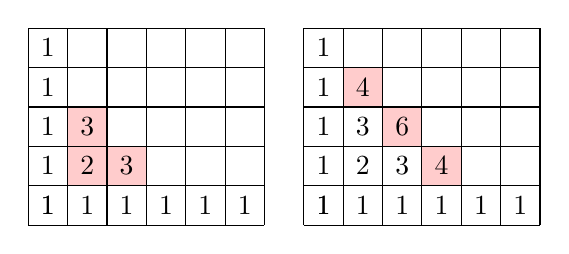
\begin{tikzpicture}[scale=.5]
      \begin{scope}
        \foreach \x in{0,1,2,3,4,5}{%
          \node at (\x + .5, .5) {1};
        }
        \foreach \x in{0,1,2,3,4}{%
          \node at (.5, \x + .5) {1};
        }
        \foreach \x/\y/\v in{1/1/2, 2/1/3, 1/2/3}{%
          \fill[color=red!20](\x,\y)rectangle(\x+1,\y+1);
          \node at (\x+.5,\y+.5){\v};
        }
        \draw(0,0)grid(6,5);
      \end{scope}
      \begin{scope}[shift={(7,0)}]
        \foreach \x in{0,1,2,3,4,5}{%
          \node at (\x + .5, .5) {1};
        }
        \foreach \x in{0,1,2,3,4}{%
          \node at (.5, \x + .5) {1};
        }
        \foreach \x/\y/\v in{1/1/2, 2/1/3, 1/2/3}{%
          %\fill[color=red!20](\x,\y)rectangle(\x+1,\y+1);
          \node at (\x+.5,\y+.5){\v};
        }
        \foreach \x/\y/\v in{3/1/4, 2/2/6, 1/3/4}{%
          \fill[color=red!20](\x,\y)rectangle(\x+1,\y+1);
          \node at (\x+.5,\y+.5){\v};
        }
        \draw(0,0)grid(6,5);
      \end{scope}
    \end{tikzpicture}
  \end{center}
  最终的结果并不重要,关键是这个过程的来源。想要知道最终结果的,可以填填看。

  这种利用表格记忆住前面步骤的结果供后面多次使用的方法,是算法中解决递归问题递归深度过大的一种常用方法。
\end{proof}